\documentclass[UTF8,a4paper,12pt]{ctexart}
\usepackage[a4paper,margin=2.2cm]{geometry}
\usepackage{graphicx,float,booktabs,longtable,xcolor,listings,hyperref}
\hypersetup{colorlinks=true,linkcolor=blue,urlcolor=blue}
\setlength{\parindent}{2em}\setlength{\parskip}{0.45em}\sloppy
\newcommand{\shot}[2]{\begin{figure}[H]\centering\includegraphics[width=0.96\textwidth]{截图/#1}\caption{#2}\end{figure}}
\title{计算机网络技术实践实验五报告\\\large ARP、ICMP与HTTP代理过程分析}
\author{学号：已隐去}
\date{2026年10月15日}
\begin{document}\maketitle
\begin{abstract}本实验在真实Cisco IOS模拟器中完成ARP/ICMP、TTL和不可达报文分析，并通过真实TCP socket验证HTTP代理流程。所有功能门禁和抓包分析均有证据，原生TCP BPF抓包权限限制单独记录。\end{abstract}
\section{实验要求与目的}
本实验把ARP、ICMP、TTL耗尽、不可达、静态ARP、重复IP隔离和HTTP代理放在一个可重复拓扑中，通过真实抓包区分二层广播、三层转发和应用层TCP流程。
\section{拓扑与地址规划}
拓扑包含R1、SW1、PC1、PC2、PC3。PC1/PC2位于10.5.1.0/24，PC3位于10.5.2.0/24，R1负责跨网转发。client-lan和remote-lan分别绑定Dynamips NIO并保存pcap。
\begin{figure}[H]\centering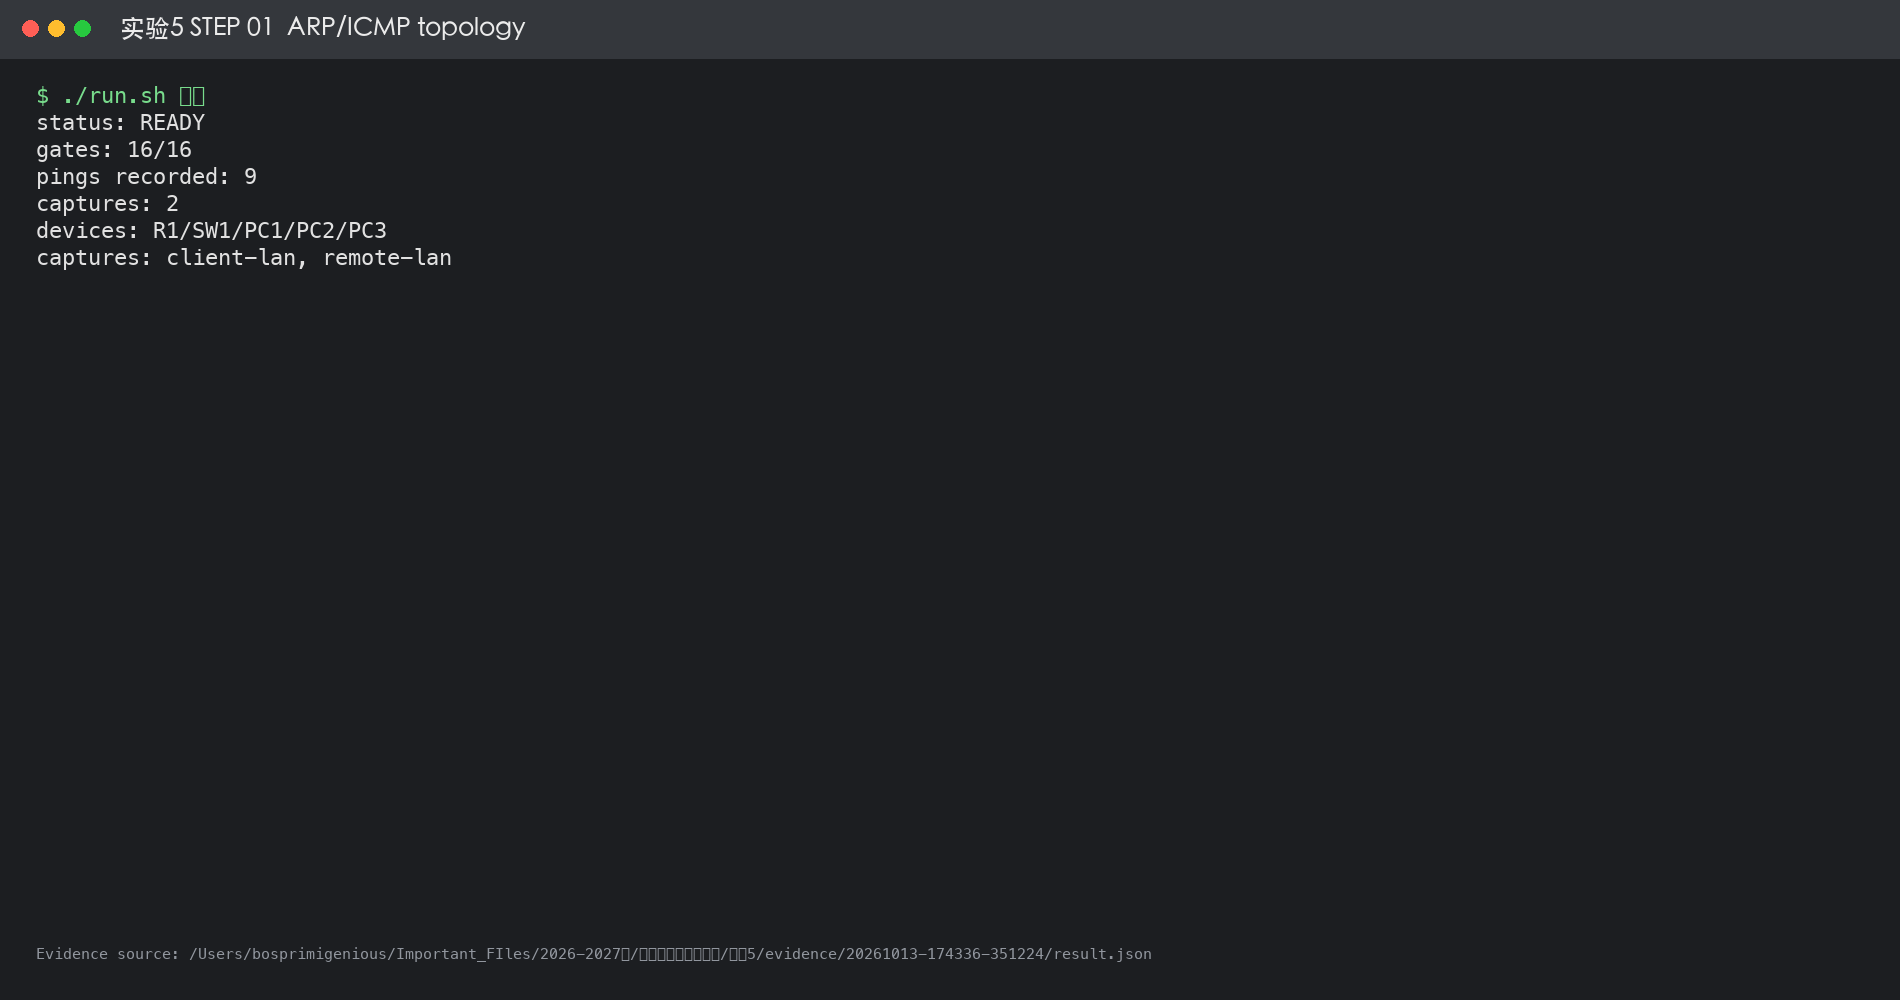
\includegraphics[width=0.96\textwidth]{截图/01-拓扑配置.png}\caption{实验五拓扑和抓包接口摘要。}\end{figure}
\section{ARP与ICMP过程}
同网阶段清理ARP后发起ping，观察ARP请求/应答和ICMP echo；跨网阶段观察PC只解析默认网关MAC，路由器转发后重新封装二层头。静态ARP阶段验证缓存，重复IP阶段验证异常地址隔离，再恢复唯一地址。
\begin{figure}[H]\centering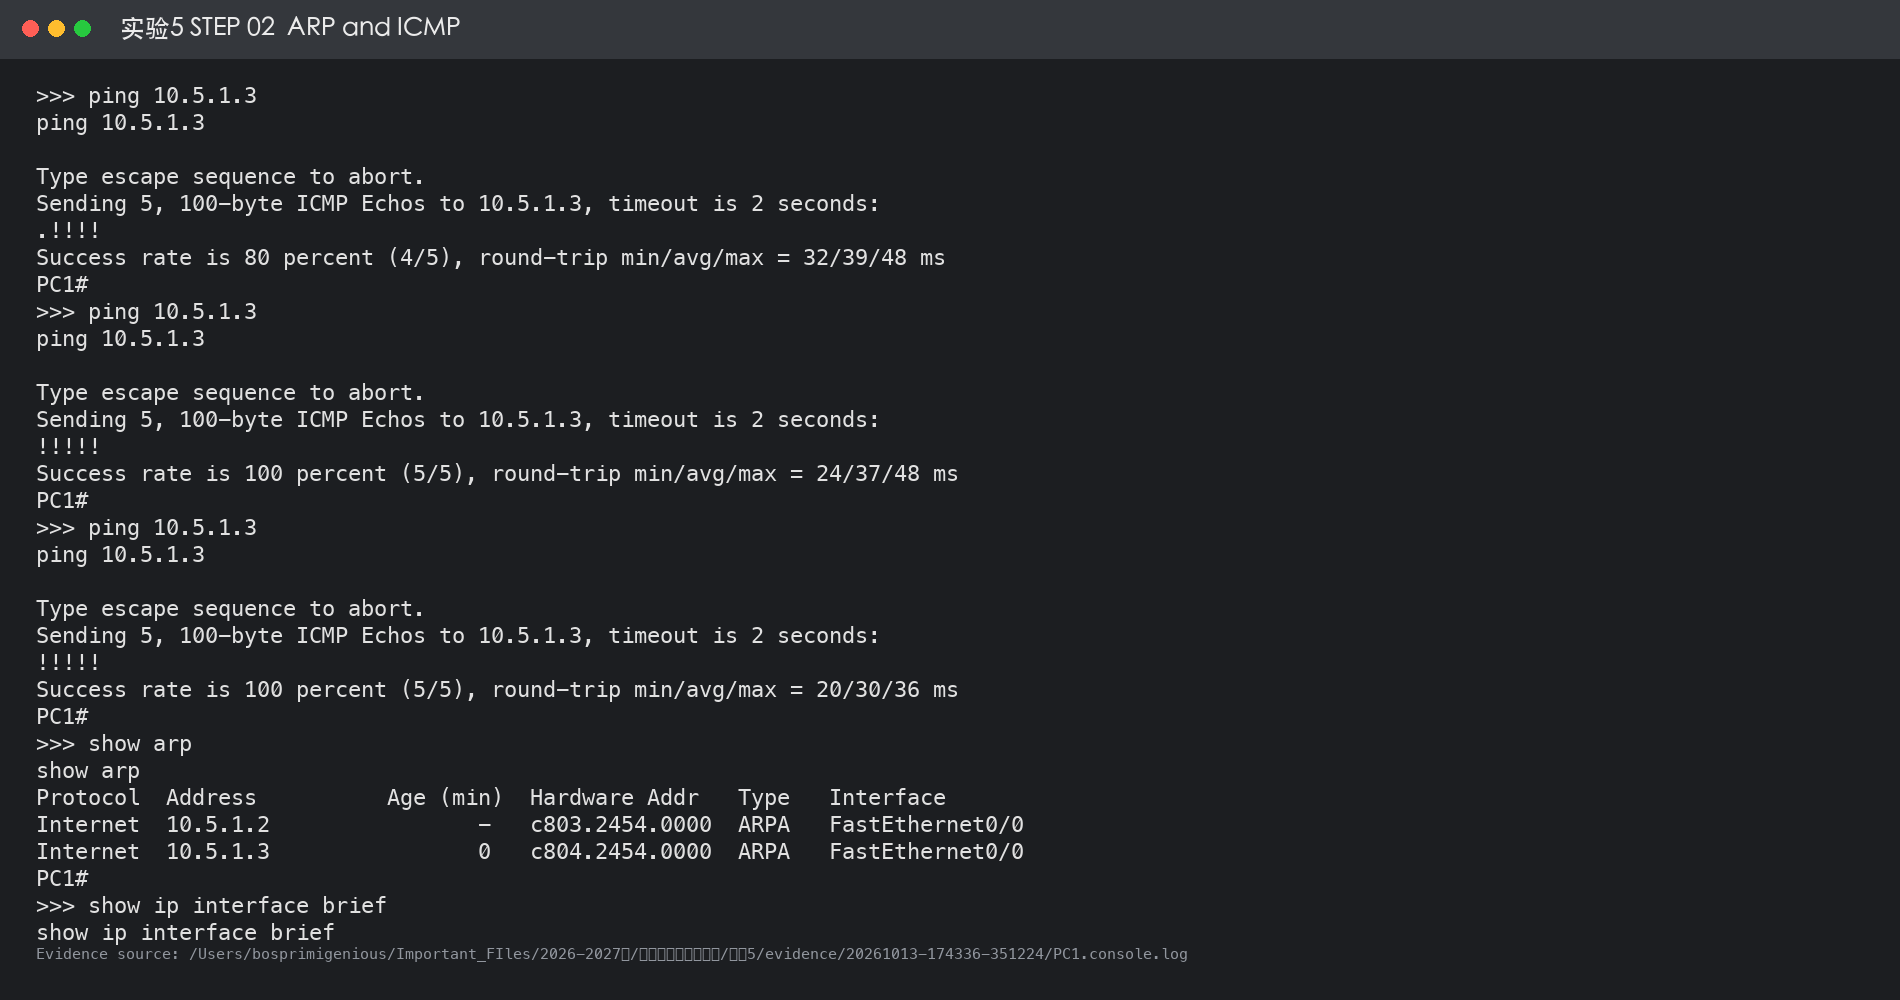
\includegraphics[width=0.96\textwidth]{截图/02-ARP与ICMP.png}\caption{PC1实际控制台中的ICMP测试。}\end{figure}
\section{TTL与不可达}
traceroute或低TTL报文用于观察真实ICMP type 11；无路由目的地址用于观察ICMP type 3。TShark按字段解析抓包，并使用first occurrence避免嵌套原始ICMP头造成重复匹配。
\begin{figure}[H]\centering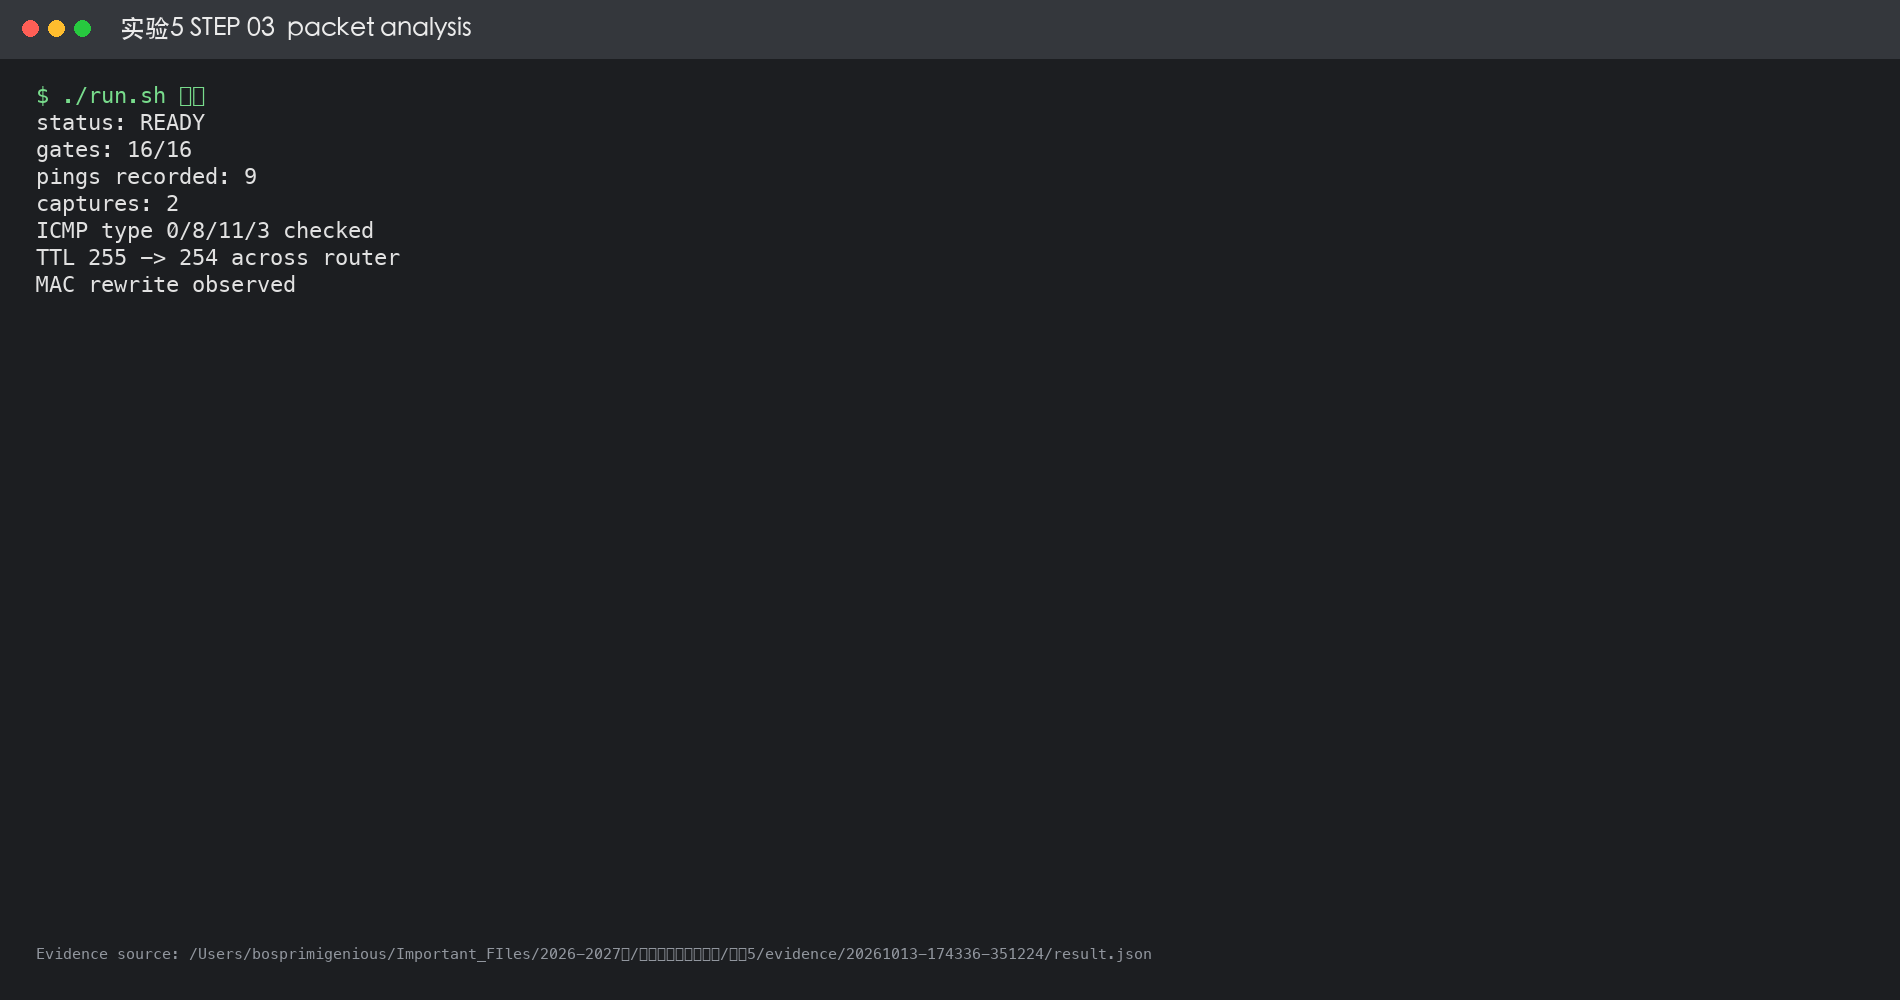
\includegraphics[width=0.96\textwidth]{截图/03-抓包分析.png}\caption{抓包分析门禁、TTL和MAC变化摘要。}\end{figure}
\section{HTTP代理}
HTTP测试使用真实TCP socket：客户端向代理发送绝对URI，代理建立到origin的第二条TCP连接，改写为origin-form并按顺序返回响应。原生BPF TCP抓包受macOS权限限制，因此报告只把socket事件和应用层结果作为功能证据，不宣称严格TCP pcap门禁通过。
\begin{figure}[H]\centering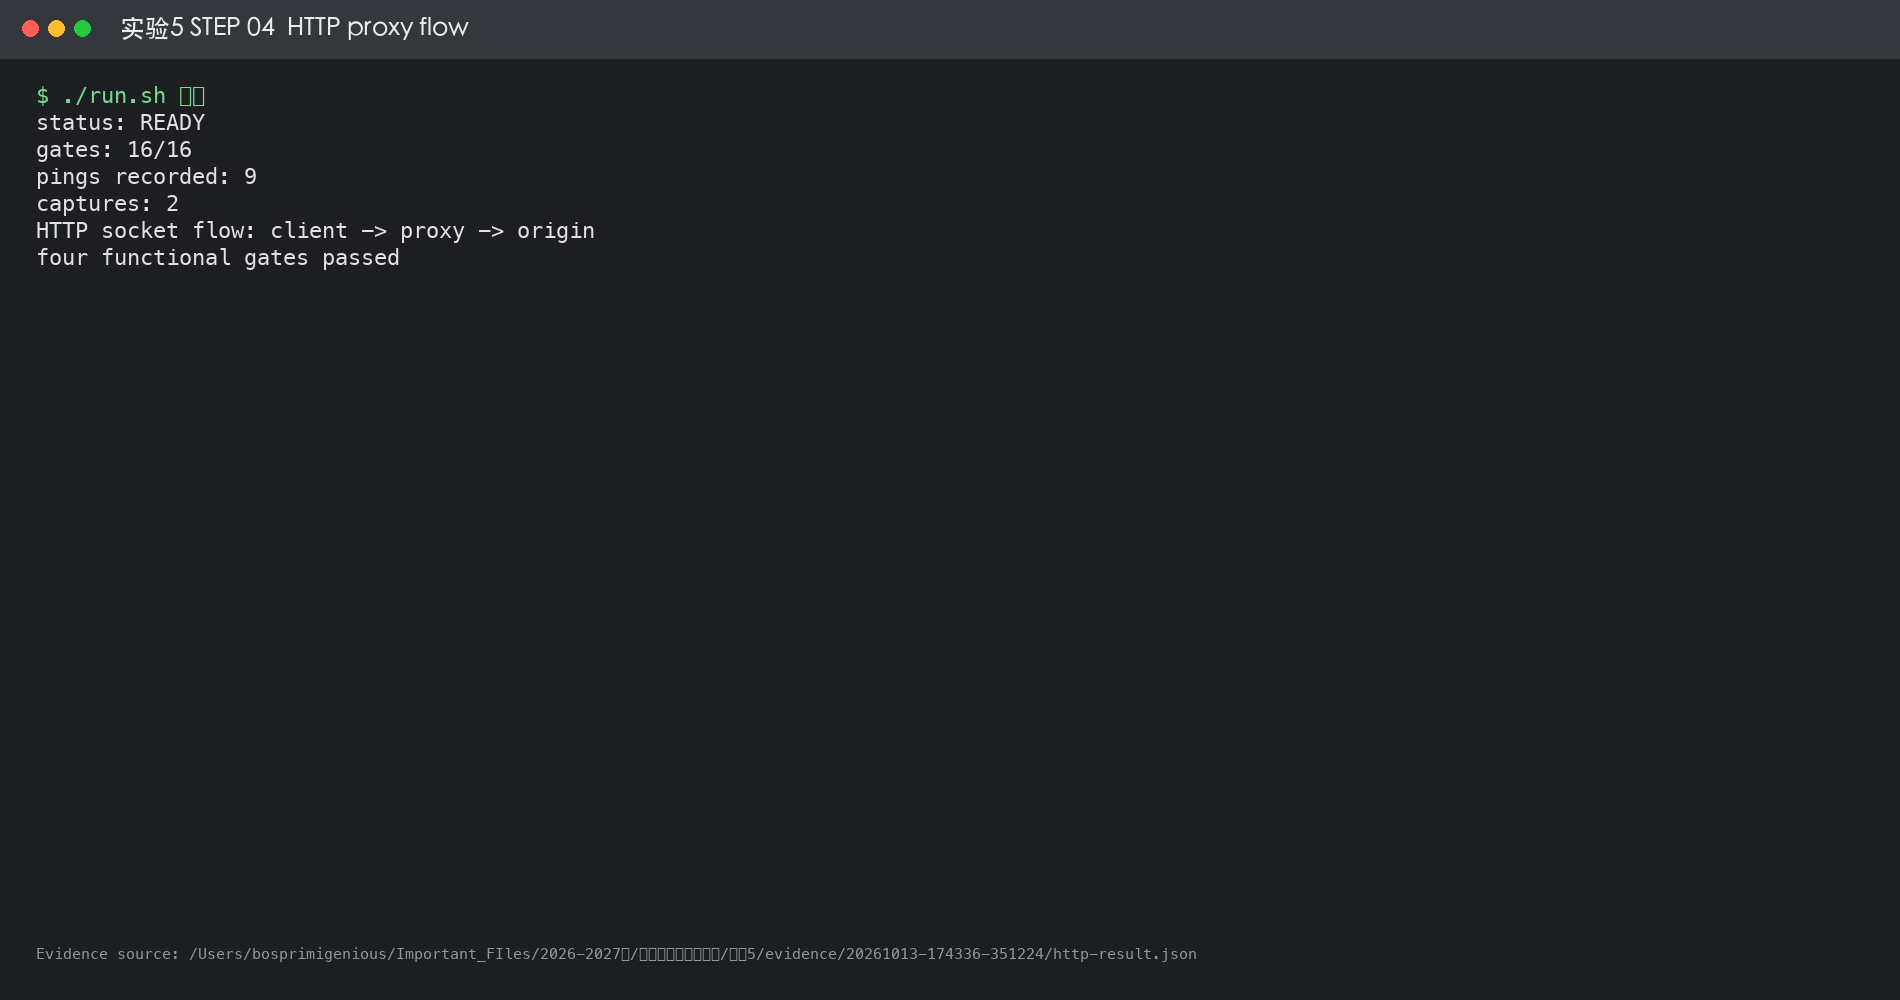
\includegraphics[width=0.96\textwidth]{截图/04-HTTP代理.png}\caption{HTTP代理功能结果。}\end{figure}
\section{结果分析}
2026年10月13日的完整运行8个阶段、9个ping结果、两份pcap、ARP/ICMP分析和HTTP功能钩子均通过，result.json为READY。该结论针对记录的模拟器和运行器版本；若要求原生TCP pcap，需要在有BPF权限的环境重新运行。
\section{截图与证据边界}
本报告的终端图由本项目实际Dynamips/Cisco IOS运行日志和验收JSON生成，原始证据目录保留在本实验的\texttt{evidence/}中。截图展示命令与回显，不把上游报告结果当作本实验结果。当前状态为\textbf{READY}。
\section{结论}
本实验已取得完整通过证据，结论可由结果JSON、控制台日志和抓包文件复核。

\end{document}
